\section{Optimizations}
\label{sec:optimizations}

\subsection{Projection Insertion}
\label{sec:field-reduction}

% Intro/Motivation 
A common optimization in data processing is to early remove intermediate values that are not needed in later phases of the computation. It has been implemented in relational databases for a long time, and has recently been added to the Pig framework. This optimization requires all field accesses in the program to be explicit. A library can provide this, but the usage is more intrusive than if the framework can use compiler support. 

% description of supported types
In \tool we support this optimization for algebraic data types, more specifically final immutable Scala classes with a finite level of nesting. Our approach does not require special syntax or access operators and supports method declarations on a data type like regular Scala classes do. While implementing our benchmarks we found this to be a reasonably expressive model for big data programming. The DSL user needs to supply class declarations, from which we generate all the necessary code for its use in \tool. For these types, LMS describes all field accesses explicitly and we can generate highly specialized code for these types including serialization schemes and other glue code for the back-ends we support.


%\todo{Drop this sentence?}The generated code includes a parsing method, to which the user simply supplies a regular expression, in case the data is stored in text form. 

% explaining the lingo and high level overview of the algorithm.
In section \ref{subsec:lms-optimizations} we have shown how LMS optimizes these classes within the same program scope. However, in \tool we endorse a declarative programming model with many short functions - each having its own scope - as these are easier to read. Each operation in our API has an input type and an output type, and they may have a parameter accepting a closure. Operations are chained together to form a data flow graph without cycles. Since types support nesting, we need to define the live values between operations as the sequence of field dereferences respective to a type to access that value. This sequence of field dereferences we call a path, and to represent it we use the scala expression needed to access it on such a type. In figure \ref{fig:type_tree} we visualize the tree which contains all paths and fields for the nested type of t in the example code in \ref{lst:types}.

For our projection insertion algorithm we need to analyze the paths on each edge of the data flow graph. We can only compute the paths for one operation when the union of all paths accessed by its successors has been already computed. For this reason we visit the graph in reverse topologically sorted order and process the operations one by one. When the successors of a node have all been processed and their paths have been propagated, that node can be analyzed to compile a list of paths it needs from its predecessors. The result of this analysis can then be used to insert projections before any operation which serializes objects or stores them in memory - we call them barriers - for example \code{cache}, \code{groupByKey} or \code{join}.

\begin{figure}
% \begin{subfigure}
\begin{lstlisting}[name=code, caption=Nested type for paths example., captionpos=b, label=lst:types]
case class A(id: String, b: B)
case class B(id: String)  
val t = ("tuple", A("a", B("b"))) 
t: scala.Tuple2[String, A]
\end{lstlisting}
% \end{subfigure}
% \begin{subfigure}
\centering
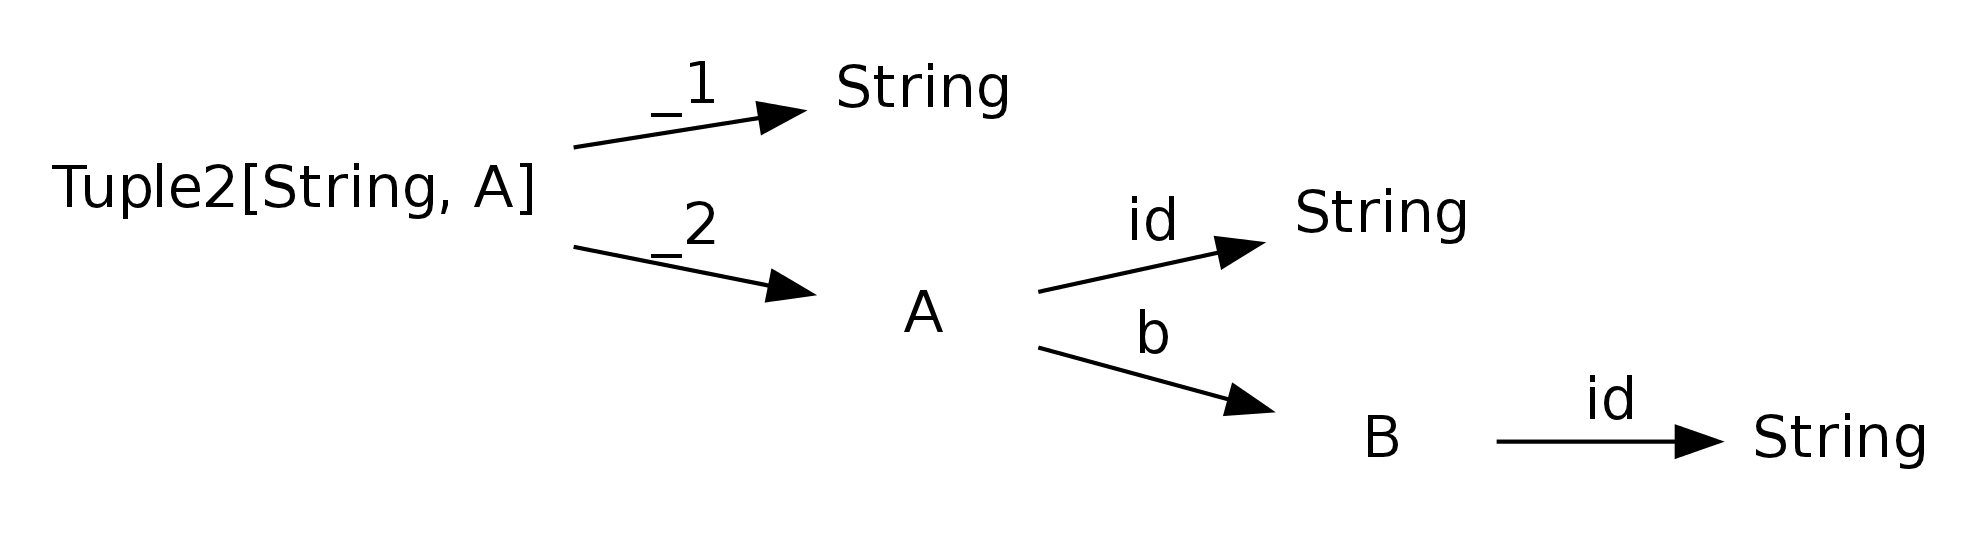
\includegraphics[clip=true, width=0.95\columnwidth]{dot/access.png}
\caption{Visualization of the nested type Tuple2[String, A]. The node labels are the types at that path, the edges describe one field dereference. The leafs are always primitive types, and the path to them is formed by concatenating the edge labels. An example path description is ``\_2.b.id''}
\label{fig:type_tree}
% \end{subfigure}
\end{figure}

% explaining the analysis

The algorithm depends on the analysis of a single operation, which we implemented using following primitives:
\begin{itemize}
\item \emph{Paths for type}: Given a type and optionally a path, this primitive creates paths for all the nested fields within. In \ref{lst:types} a \code{save} with element type A returns the paths \code{id} and \code{b.id}. 
\item \emph{Closure analysis}: This primitive returns a list of all paths accessed in a closure that read (recursively) from the closure's input.
\item \emph{Rewrite paths}: Several operations have defined semantics which influence the type and therefore the paths. For example, the \code{cache} operation will always have the same input and output type and is known to return the same instance, so all paths from it's successors must be propagated to its predecessors. The \code{groupByKey} operation on the other hand always reads all parts of the key, and has to rewrite all paths of the form \code{\_2.iterable.x} to \code{\_2.x}, as the iterable is introduced by the operation itself and is known to conserve the instances.
\item \emph{Narrow closure}: Given a list accessed paths and a closure, this primitive replaces the closure's original output symbol with one that reads from it and creates a new object only containing the fields needed for later stages.
\end{itemize}

For \code{map} operations which output a nested type we need to combine the narrow closure and the closure analysis primitive. SOA ensures that the output symbol of a closure is always a constructor invocation for these. We then use the narrow closure primitive to create a new closure, in which the output symbol reads from the old output symbol. LMS recognizes a field read that reads from a constructor invocation in the same scope and optimizes this by reading the value that was used to initialize the field directly. This happens for all the fields, if the corresponding constructor invocation is in the same scope. Therefore the old constructor invocation will not be read anymore, and DCE will pick it up. This means that the field values only it was reading will also not be read anymore, and they too will be eliminated. Then we can analyze this new closure to get the accessed paths from it. 

Table \ref{table:field_reduction} shows how these primitives are combined to form the rules for the most important operations in our API.

 \begin{table}[width=0.5\pagewidth]

    \begin{tabularx}{0.5\textwidth}{l|X|l}
        operation    & Propagate accessed paths 							     & barrier \\ \hline
        filter       & All of successor + closure reads                                                      & ~       \\ 
        flatMap      & All of the closure with a replaced output                                             & ~       \\ 
        map          & All of the closure with a replaced output                                             & ~       \\ 
        join         & All paths for the key, rewrites accesses to values to the correct predecessor         & x       \\ 
        groupByKey   & All paths for the key, rewrites accesses to the value's iterable to the value itself  & x       \\ 
        reduce       & All accesses from the closure are translated to access of the value's iterable        & ~       \\ 
        save         & All paths for input type           	                                             & ~       \\ 
    \end{tabularx}
    
    \caption{Access path computation and propagation for selected operations.}
\label{table:field_reduction}
 \end{table}

